\section{Manuel Gómez Hernández}
\subsection{Definiciones}

\begin{enumerate} 
\item \textbf{La'tex: }
     \\Sistema de composición tipografica de alta calidad.

\item \textbf{GitHub: }
    \\Forja para alojar proyectos utilizando el sistema de control de git.

\item \textbf{git: }
    \\Sistema de control de versiones distrubuido, lo que significa que es un clon local de proyectos, es un repositorio de control de versiones completas.

\item \textbf{Precision: }
    \\Es la variación, disperción, poca variación, significa un buen grado de precisión.

\item \textbf{Exactitud: }
    \\Se define con respecto a su cercania (sesgo), mayor cercania implica un buen grado de exactitud.

\item \textbf{Estudio: } 
\begin{enumerate}
\item Esfuerzo que pone el entendimiento aplicándose a conocer algo.
\\ \textit{Análisis, investigación, observación, examen.}
\item Trabajo empleado en aprender y cultivar una ciencia o arte.
\\ \textit{Aprendizaje, formación, instrucción, preparación, enseñanza, aplicación, memorización.}
\cite{RAE}
\end{enumerate}

\item \textbf{Trabajo: }
\begin{enumerate}
    \item Acción y efecto de trabajar.
    \\ \textit{Labor, faena, brega, operación, curro, curre, currelo.}
    \item Ocupación retribuida.
    \\ \textit{Empleo, oficio, profesión, ocupación, cargo, puesto, plaza, función, chamba.}
    \item Cosa que es resultado de la actividad humana.
    \\ \cite{RAE}
\end{enumerate}

\item \textbf{Estudio de movimientos y tiempos: }
\\ Es el análisis de métodos, materiales, herramientas e instalación utilizada o que se ha de utilizar en la ejecución de un trabajo.
\\ \cite{DiapositivasSema-2-21}

\item \textbf{Análisis: }
\begin{enumerate}
    \item Distinción y separación de las partes de algo para conocer su composición.
    \\ \textit{Expliración, investigación, observación.}
    \item Estudio detallado de algo, especialmente de una obra o de un escrito.
    \\ \textit{Estudio, examen.}
    \\ \cite{RAE}
\end{enumerate}

\item \textbf{Sistema: }
\begin{enumerate}
    \item Conjunto de reglas o principios sobre una materia racionalmente enlazados entre sí.
    \\ \textit{Método, procedimiento, plan, manera, forma, modo, medio, técnica.}
    \item Conjunto de cosas que relacionadas entre sí ordenadamente contribuyen a determinado objeto.
    \\ \textit{Ordenación, organización, estructura, taxonomía.}
    \\ \cite{RAE}
\end{enumerate}

\item \textbf{Tiempo: }
\begin{enumerate}
    \item Duración de las cosas sujetas a mudanza.
    \\\textit{Duración.}
    \item Magnitud física que permite ordenar la secuencia de los sucesos, estableciendo un pasado, un presente y un futuro, y cuya unidad en el sistema internacional es el segundo.
    \item Parte de la secuencia de los sucesos.
    \\ \cite{RAE}
\end{enumerate}

\item \textbf{Predeterminar: }
\begin{enumerate}
    \item Determinar o resolver con anticipación algo.
    \\ \textit{Preestablecer, prefijar, estipular, preconcebir}
    \\ \cite{RAE}
\end{enumerate}

\item \textbf{Sistemas de tiempo predeterminado (STP): }
    \\ Conjunto de reglas o métodos para determinar con anticipación la secuencia de sucesos.
    \\ \cite{DiapositivasSema-2-21}

\item \textbf{Estudio de micromovimientos: }
    \\Division de la asignación de trabajo en therbligs que se logra mediante el analisis, cuadro por cuadro de una pelicula y la mejora de la operación a traves de la eliminación de los movimientos innecesarios y la simplificación de los necesarios.

\item \textbf{Estudio de metodos: }
    \\factores fundamentales en la determinación de la productividad de los operarios.

\item \textbf{MTM: }
    \\Métodos de medición del tiempo.
    \\Medición de tiempos de métodos.
    \\ \cite{DiapositivasSema-2-22}

\item \textbf{TMU: }
    \\Unidades de medida de tiempo.
    \\ \cite{DiapositivasSema-3-27}

\item \textbf{(1)Alcanzar (Reach "R"): }
    \\Por alcanzar se entiende el movimiento realizado con la mano vacía.
    \\ \cite{DiapositivasSema-3-27}

\item \textbf{(2)Mover (Move "M"): }
    \\Se refiere al movimiento con un objeto en la mano.
    \\ \cite{DiapositivasSema-3-27}

\item \textbf{FD: }
    \\Fáctor dinámico.
    \\ \cite{DiapositivasSema-3-27}

\item \textbf{CE-TMU: }
    \\Constante estática TMU.
    \\ \cite{DiapositivasSema-3-27}

\item \textbf{Muestreo: }
    \begin{enumerate}
        \item Acción de escoger muestras representativas de la caludad o condiciones meidias de un todo.
        \item Técnica empleada en un muestreo.
        \item Selección de una pequeña parte estadísticamente determinada, utilizada para inferir el valor de una o varias características del conjunto.
        \\ \textit{Unidad de muestreo.}
        \\ \cite{DiapositivasSema-4-04}
    \end{enumerate}

\item \textbf{Representativo, va: }
\begin{enumerate}
    \item Que sirve para representar algo.
    \\ \textit{Característico, propio, peculiar, específico, clásico, típico, individual.}
    \item Que representa con justos títulos.
    \\ \textit{Relevante, significativo, importante.}
    \\ \cite{RAE}
\end{enumerate}

\item \textbf{Infeir: }
\begin{enumerate}
    \item Deducir algo o sacarlo como conclusión de otra cosa.
    \\\textit{Deducir, derivar, concluir, colegir, inducir.}
    \item Producir un daño físico o moral.
    \\ \textit{Infligir, dañar, lastimar, herir.}
    \item Incluir o llevar consigo algo.
    \\ \cite{RAE}
\end{enumerate}

\item \textbf{Muestreo: }
    \\Acción de escoger muestras que describan de manera exacta las características de un conjunto de datos que permitirán deducir y sacar conclusiones del fenómeno a estudiar.
    \\ \cite{DiapositivasSema-4-04}

\item \textbf{Muestro del trabajo: }
    \\Herramienta para disminuir el costo que se presenta en el estudio continuo del tiempo.
    \\ \cite{DiapositivasSema-4-04}

\item \textbf{Muestreo discreto: }
    \\Implica seleccionar elementos específicos de una población finita o contable, donde cada elemento tiene una probabilidad asociada de ser elegido.
    
\item \textbf{Muestreo continuo: }
    \\Selección de elementos de una población infinita, donde los valores pueden tomar cualquier valor dentro de un rango específico, como la altura o el tiempo.

\item \textbf{Estudio de tiempos convencional: }
    \\Es una muestra continua de n ciclos (Suponiendo que la distribución estadística es normal).
    \\ \cite{DiapositivasSema-4-04}

\item \textbf{Distribución estadística normal: }
    \\Forma de distribución estadística simétrica con forma de campana, donde la mayoría de los datos se concentran cerca de la media.

\item \textbf{Estudio de tiempos no convencional: }
    \\Es una muestra discreta (Suponiendo que la distribución estadística es binomial).
    \\ \cite{DiapositivasSema-4-04}

\item \textbf{Distribución estadística binomial: }
    \\Modelo estadístico que describe la probabilidad de obtener un número específico de éxitos en un número fijo de ensayos independientes, donde cada ensayo tiene dos resultados posibles: éxito o fracaso.

\item \textbf{Pronostico: }
    \\Valor que se cree obtener.
    
\item \textbf{Estimación: }
    \\Analisis a traves de operaciones.

\end{enumerate}

\subsection{Materiales}


\subsubsection{Tabla de materiales}

\subsubsection{Trazado de Materiales }

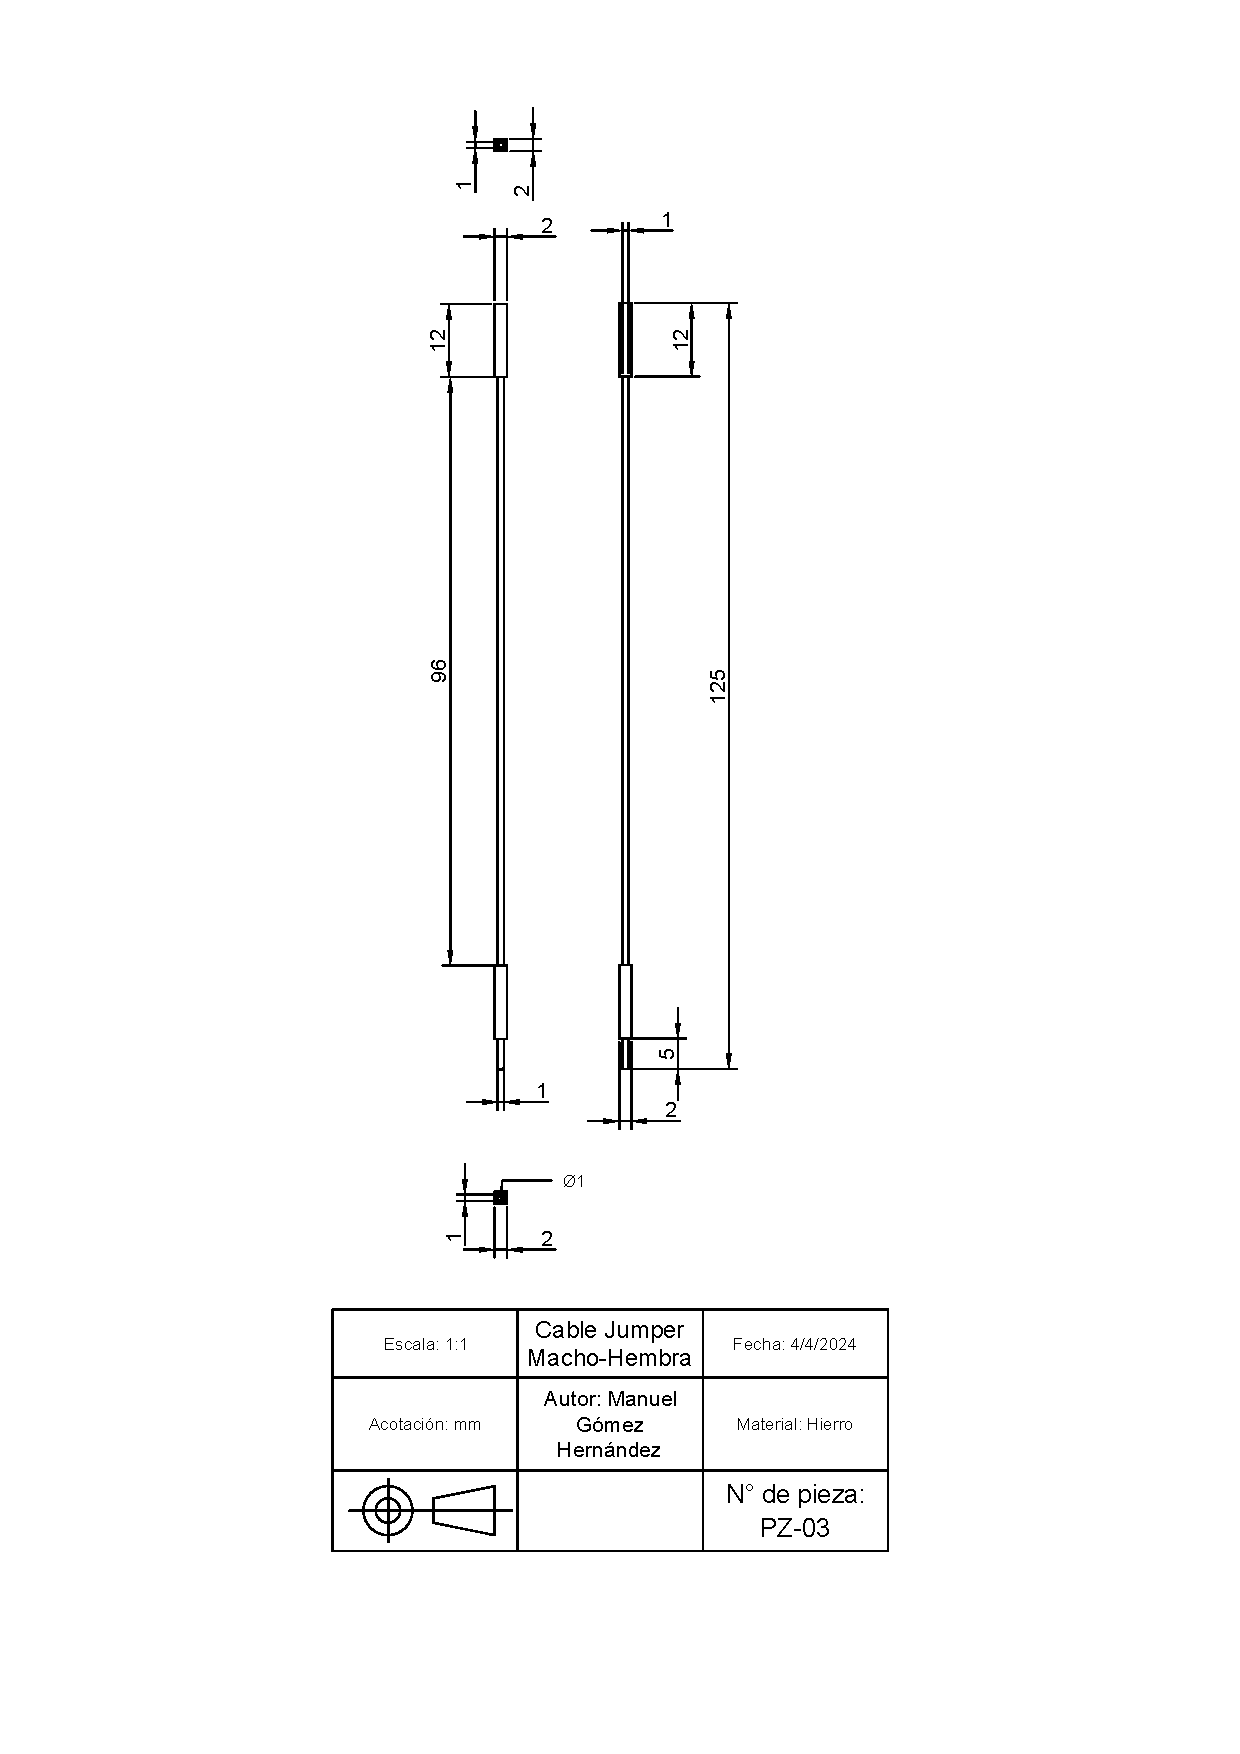
\includegraphics[width=.9\textwidth]{15/img/cableJumperMHTrazo.pdf}~\\[15cm]
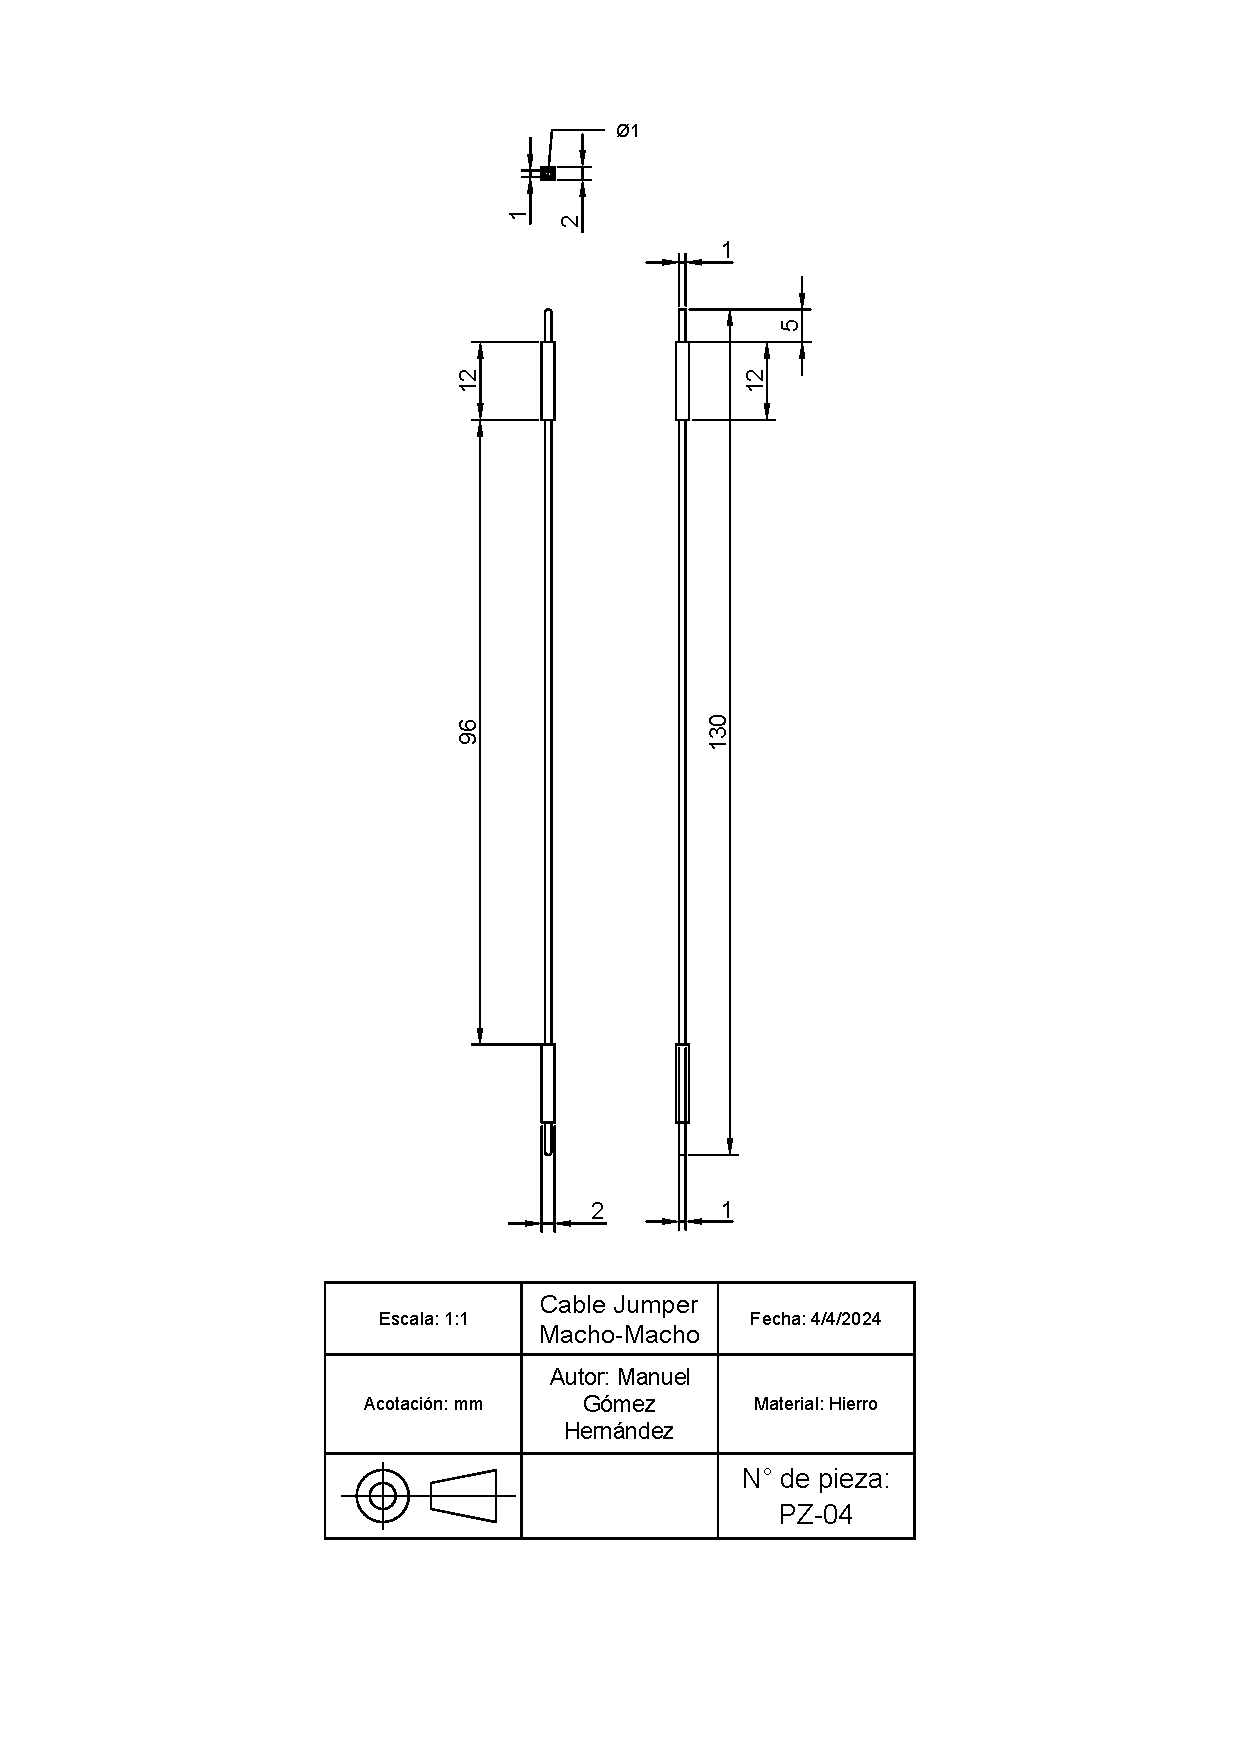
\includegraphics[width=.9\textwidth]{15/img/cableJumperMMTrazo.pdf}~\\[15cm]
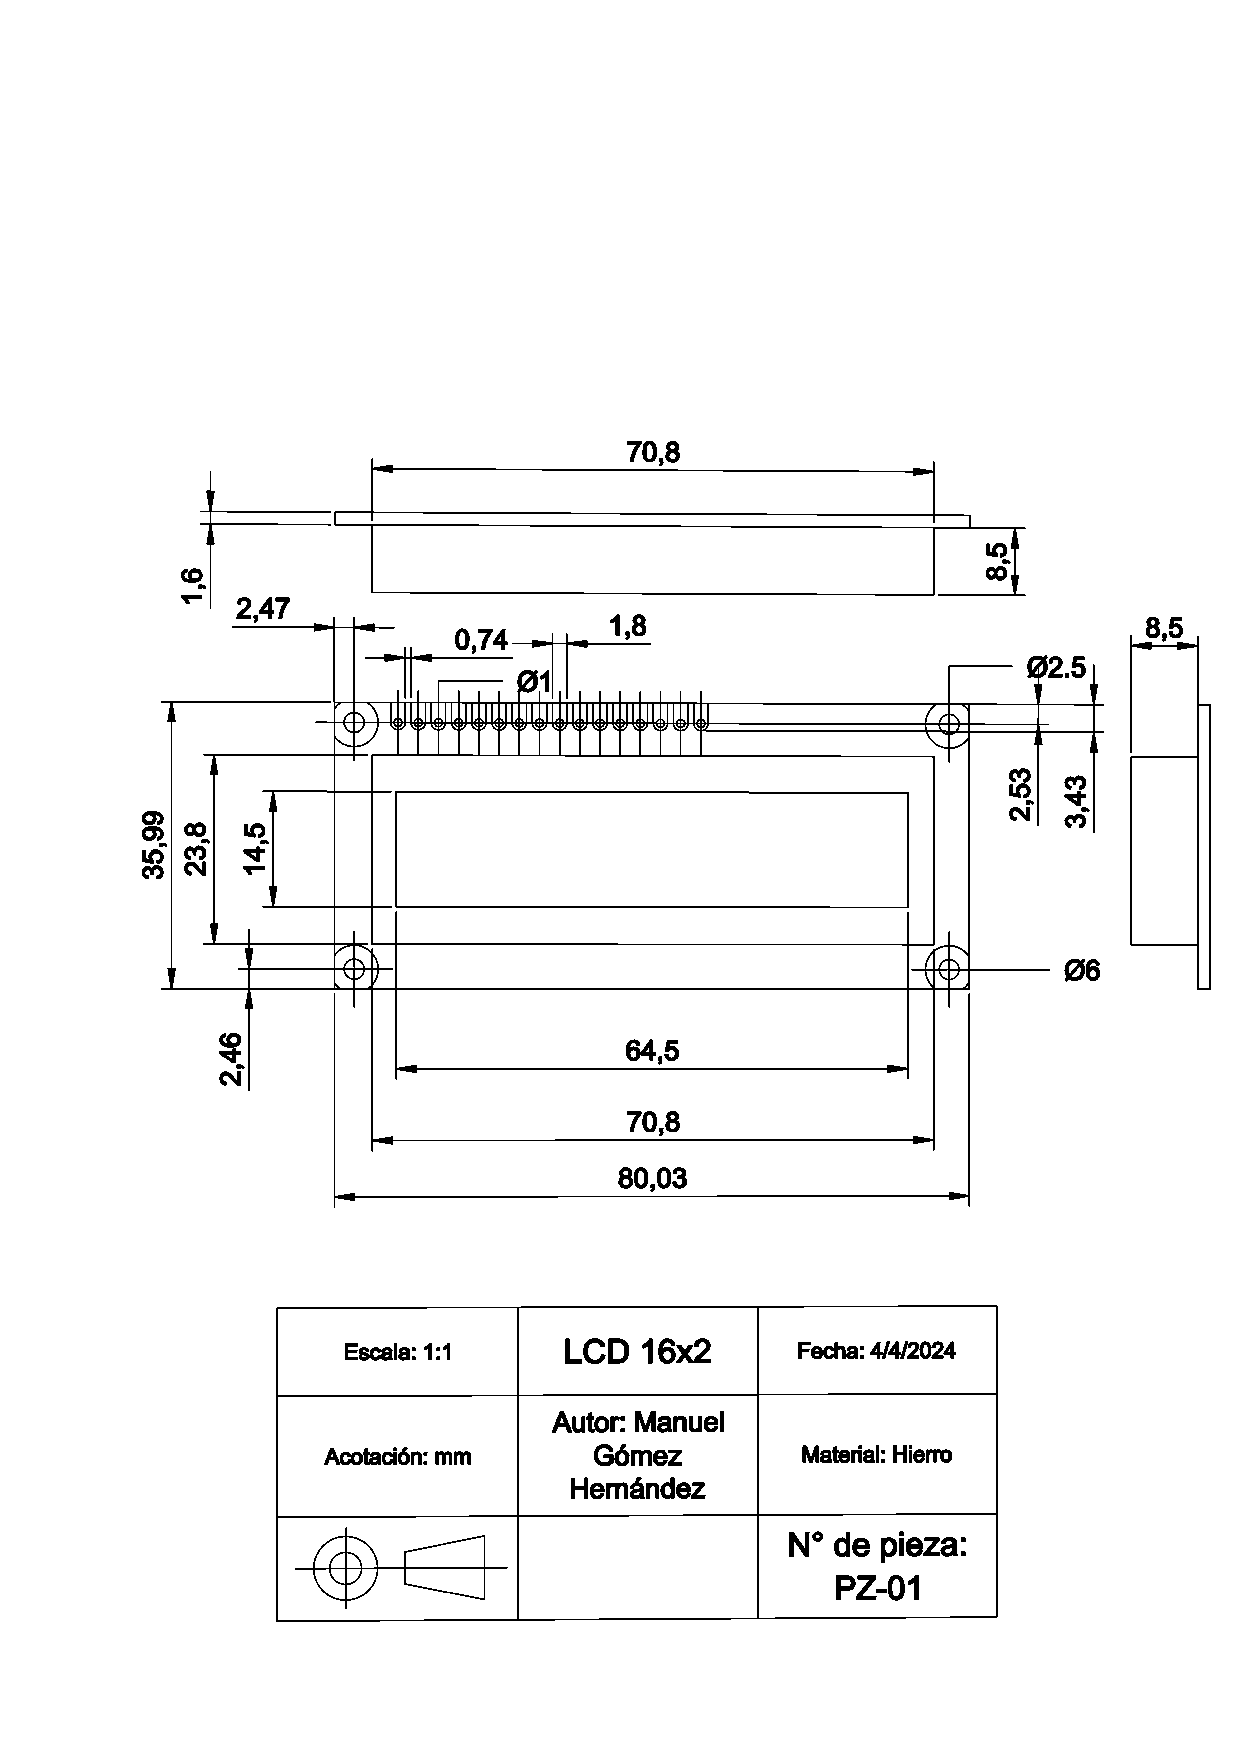
\includegraphics[width=.9\textwidth]{15/img/lcdTrazo.pdf}~\\[15cm]
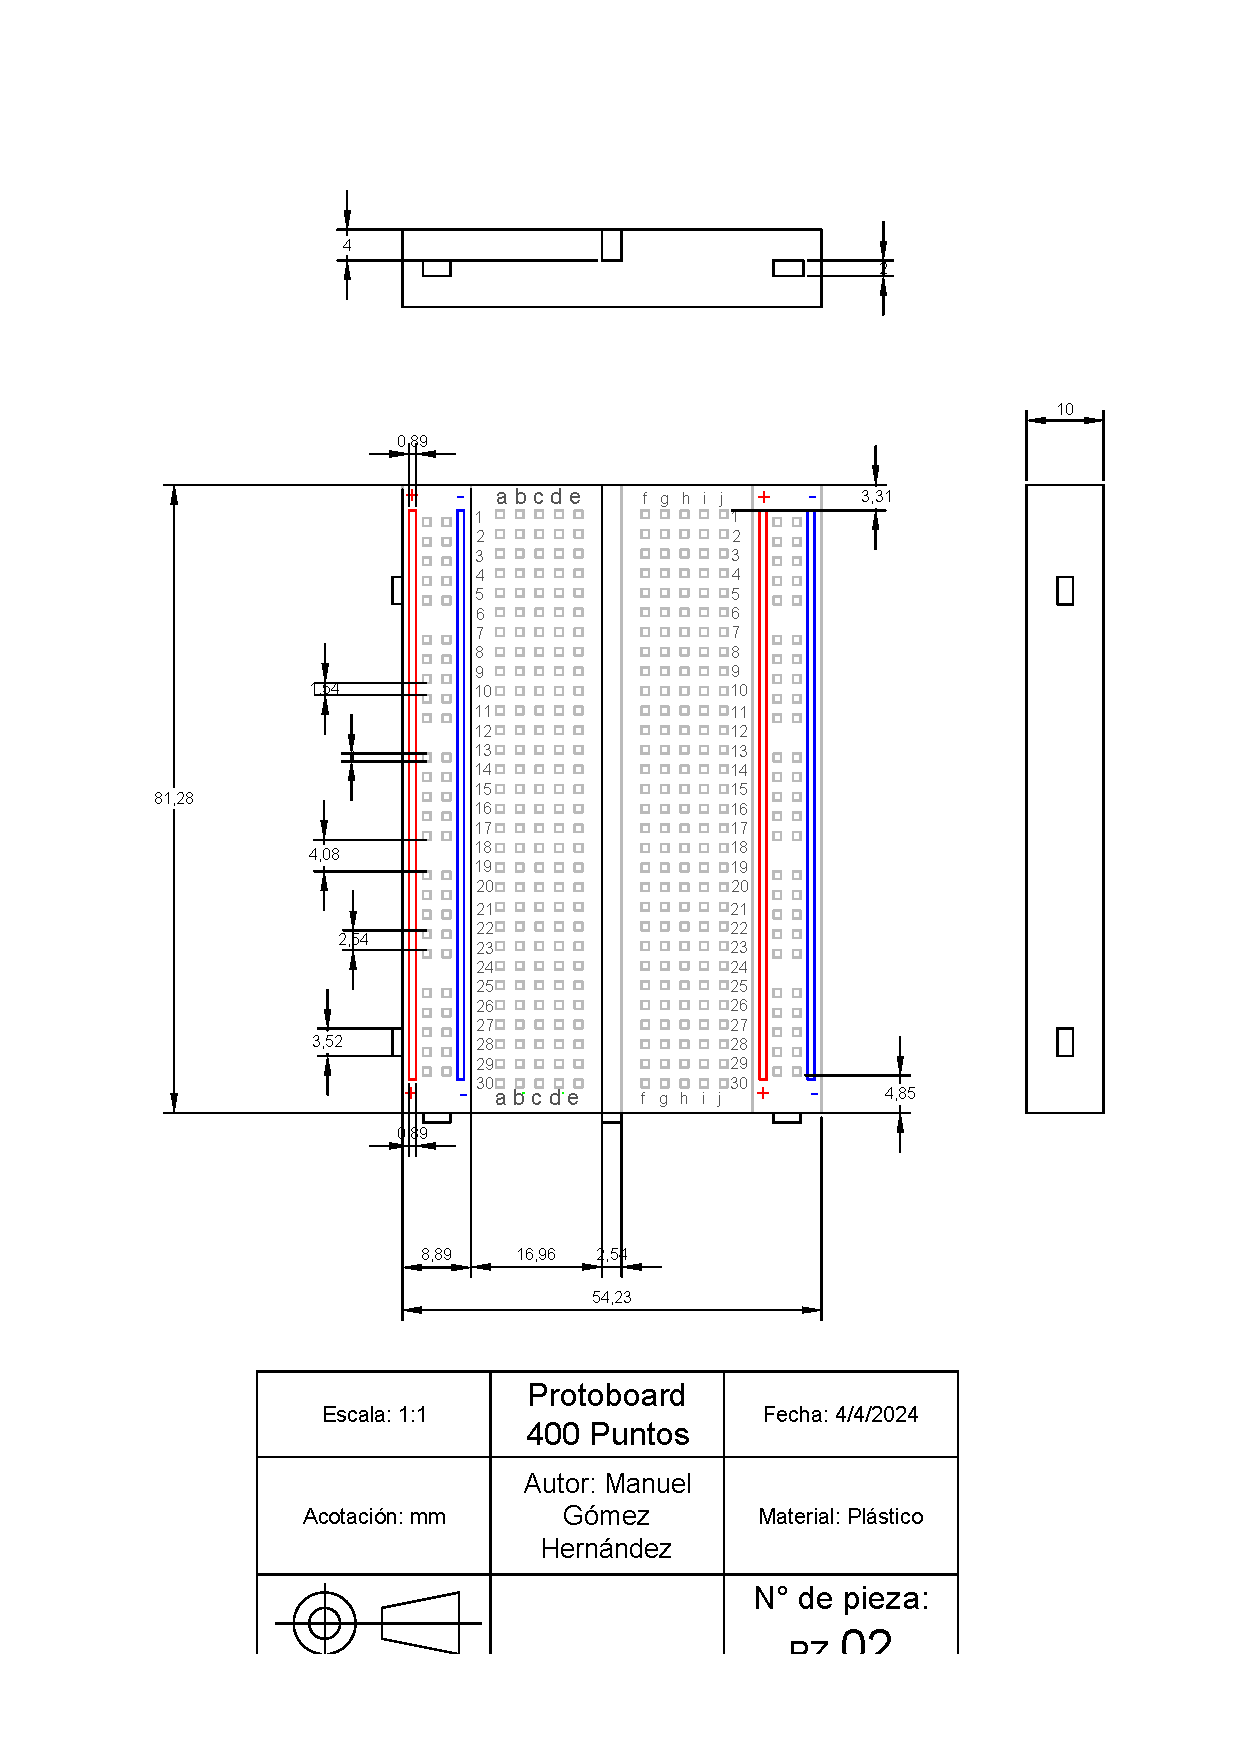
\includegraphics[width=.9\textwidth]{15/img/placaProtoboardTrazo.pdf}~\\[15cm]
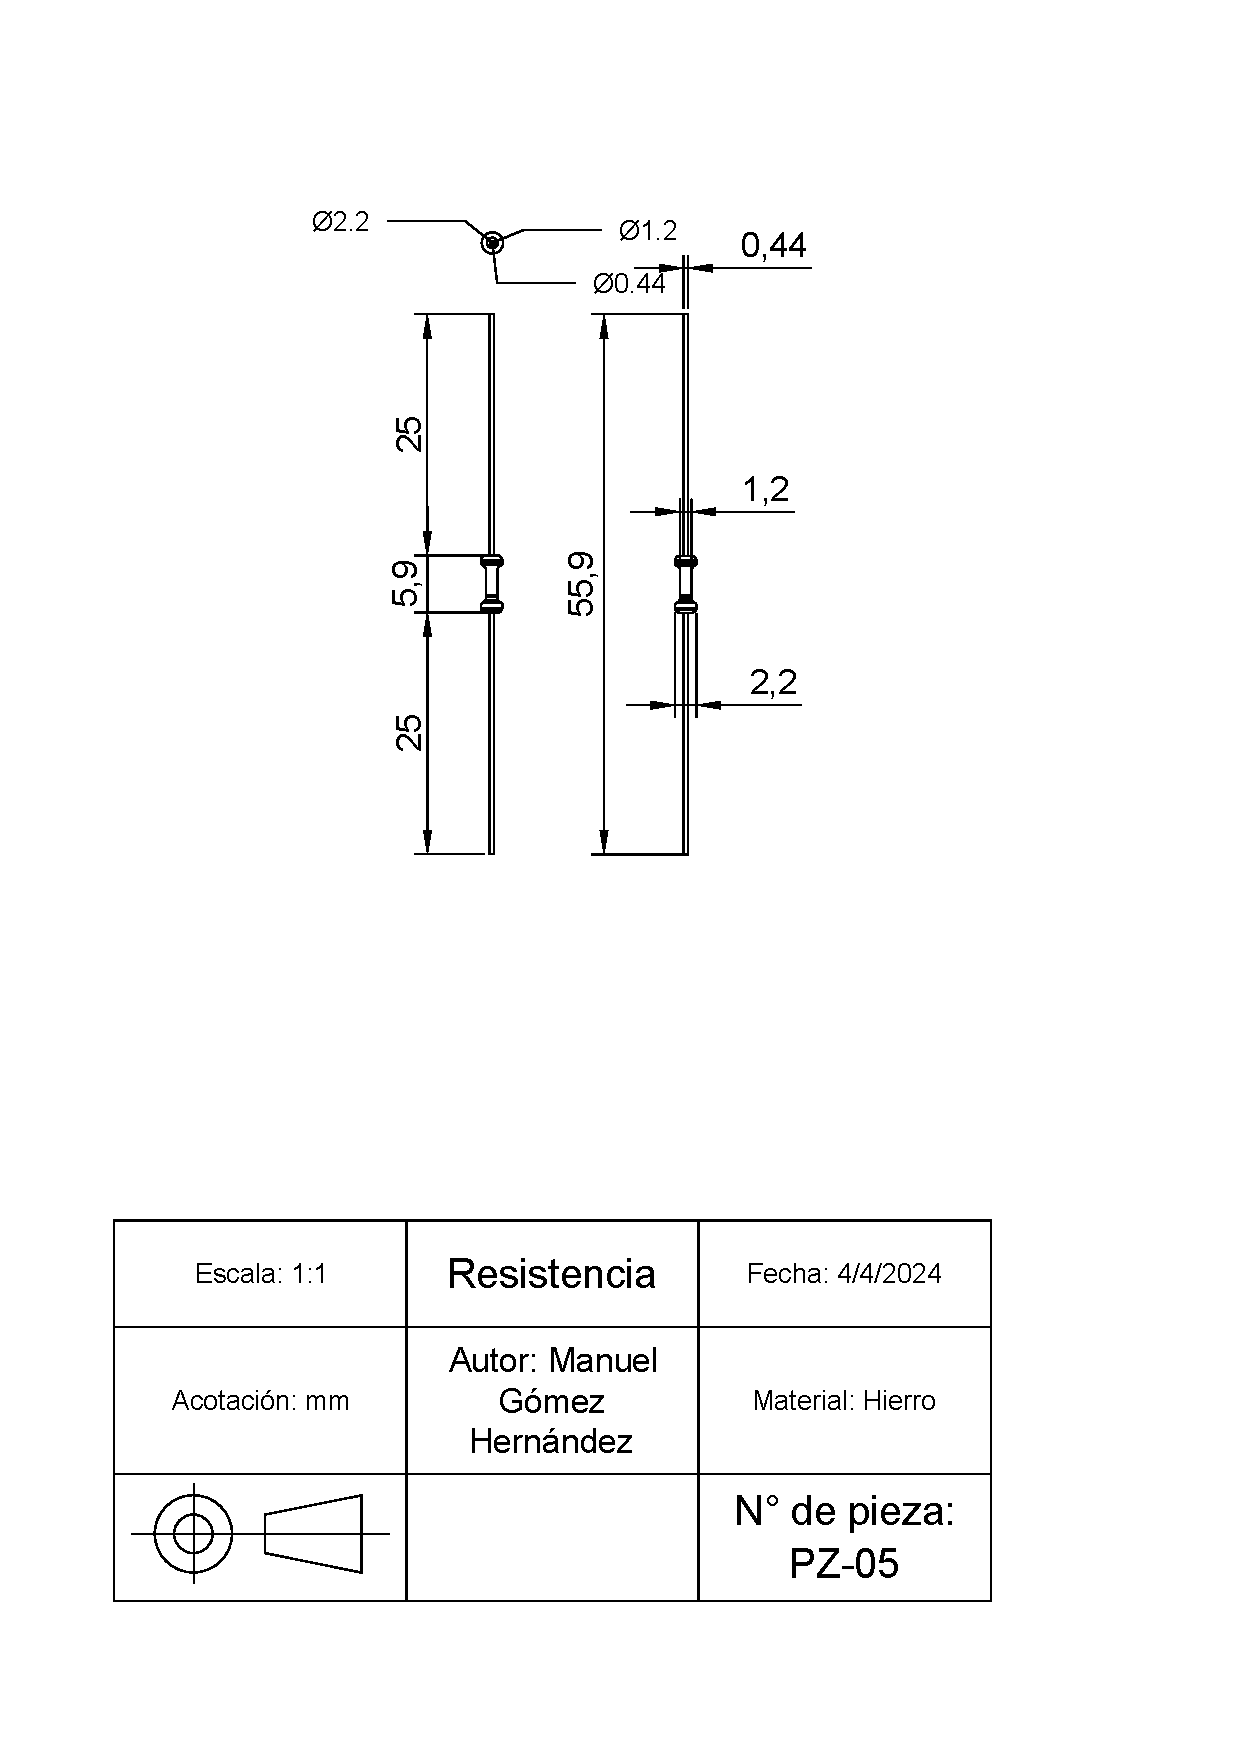
\includegraphics[width=.9\textwidth]{15/img/resistenciaTrazo.pdf}~\\[15cm]




\bibliographystyle{apalike}
\bibliography{15/referencias}

